
\section{Architecture of Histo}
\label{sec:main.histo}

Based on the requirements and the evaluation of CouchDB we derive a new architecture for a practical synchronization solution.

\begin{itemize}
\item
  \textbf{No Timestamps}: history-based 3-way merging
\item
  \textbf{No Change Tracing}: explicit change tracing is not necessary - support
  diff computation on the fly
\item
  \textbf{Data Agnostic}: leave diff and merge of the actual data to
  plugins
\item
  \textbf{Distributed}: synchronization does not require a central server
\item
  \textbf{Functional Design}: only implement the functional parts of synchronization - leave everything else to the application (transport, persistence)
\item
  \textbf{Sensitive Defaults}: have defaults that `just work' but
  still support custom logic (e.g. for conflict resolution)
\item
  \textbf{Cross-Platform}: be available on every major platform through the use of Web Standards
\end{itemize}

\section{Hierarchical Data Model Mapping}
Our data described in the scenario is structured through entity instances, their attribute values and relationships to other instances.
Most modern web application frameworks realize one-to-one relationships by simply having an attribute storing the related instance's ID.
One-to-many relationships are realized through an attribute having a collection of 
instance IDs as its value.\\
Instance collections often have a relevant order that needs to be preserved.
An example is the list of tasks in a project that is displayed to the user.
The user wants to be able to change the order of tasks and the order should be persisted.\\
We further differentiate between linking to a separately stored instance and  embedding an instance.
An embedded instance can still be linked from other instances but it cannot be embedded twice.
Linking to an instance means to simply hold another instance's ID as an attribute value, embedding means to hold both their ID and actual state.\\

The merge and commit processes, described in the next sections, depend on a hierarchical representation of our application state.
To have a hierarchy we need to define a single root structure from where all substructures of our state can be reached.\\
Our hierarchical structure can be as simple as this:

\begin{itemize}
\item Level 0 (Root): list of entities
\item Level 1: list of instances per entity
\item Level 2: list of attributes per instance
\end{itemize}

This gives us a very flat tree with each entity node linking to a potentially large number of instances.
For example, our comments entity would directly link to all comments across all projects and tasks.
The next sections will show that it is beneficial for merging performance if each tree node only links to a small number of child nodes.\\
This is where the difference between linking and embedding comes into play.
We can achieve a deeper hierarchy by embedding certain instances in others.
In our scenario we could decide to embed tasks inside projects through one of its attributes.
Comments could in turn be embedded inside tasks.\\
In order to develop a merging algorithm we need to map each substructure of our hierarchy to a suitable data structure.\\
Starting at the top we choose the list of projects as the root structure of our data.
The project list is represented through a \emph{dictionary} embedding all project instances.
The dictionary keys are the instance IDs and the dictionary values embed the actual instances.\\
Each instance is again represented through a \emph{dictionary}.
The dictionary keys correspond to the attributes and the dictionary values to attribute values.\\
If the attribute values are atoms, the hierarchy stops here.
Attributes with string values can be represented with \emph{ordered lists}.
Attribute values linking to other instances are represented through \emph{(ordered) sets}.
We can choose a set as the list can only contain unique instance IDs.\\
Attribute values embedding other instances are represented through an \emph{(ordered) dictionary}.
Like in our project list at the beginning, keys are the IDs of instances and values their actual state.\\
If other instances are embedded, they are kept as children in the hierarchy.\\

Let us summarize the full mapping between model elements and data structures:

\begin{itemize}
\item Instances and their attributes: dictionaries
\item String values: ordered lists
\item Collections linking to instances: (ordered) sets
\item Collections embedding instances: (ordered) dictionaries
\end{itemize}

\begin{figure}[hierarchy]
  \centering
  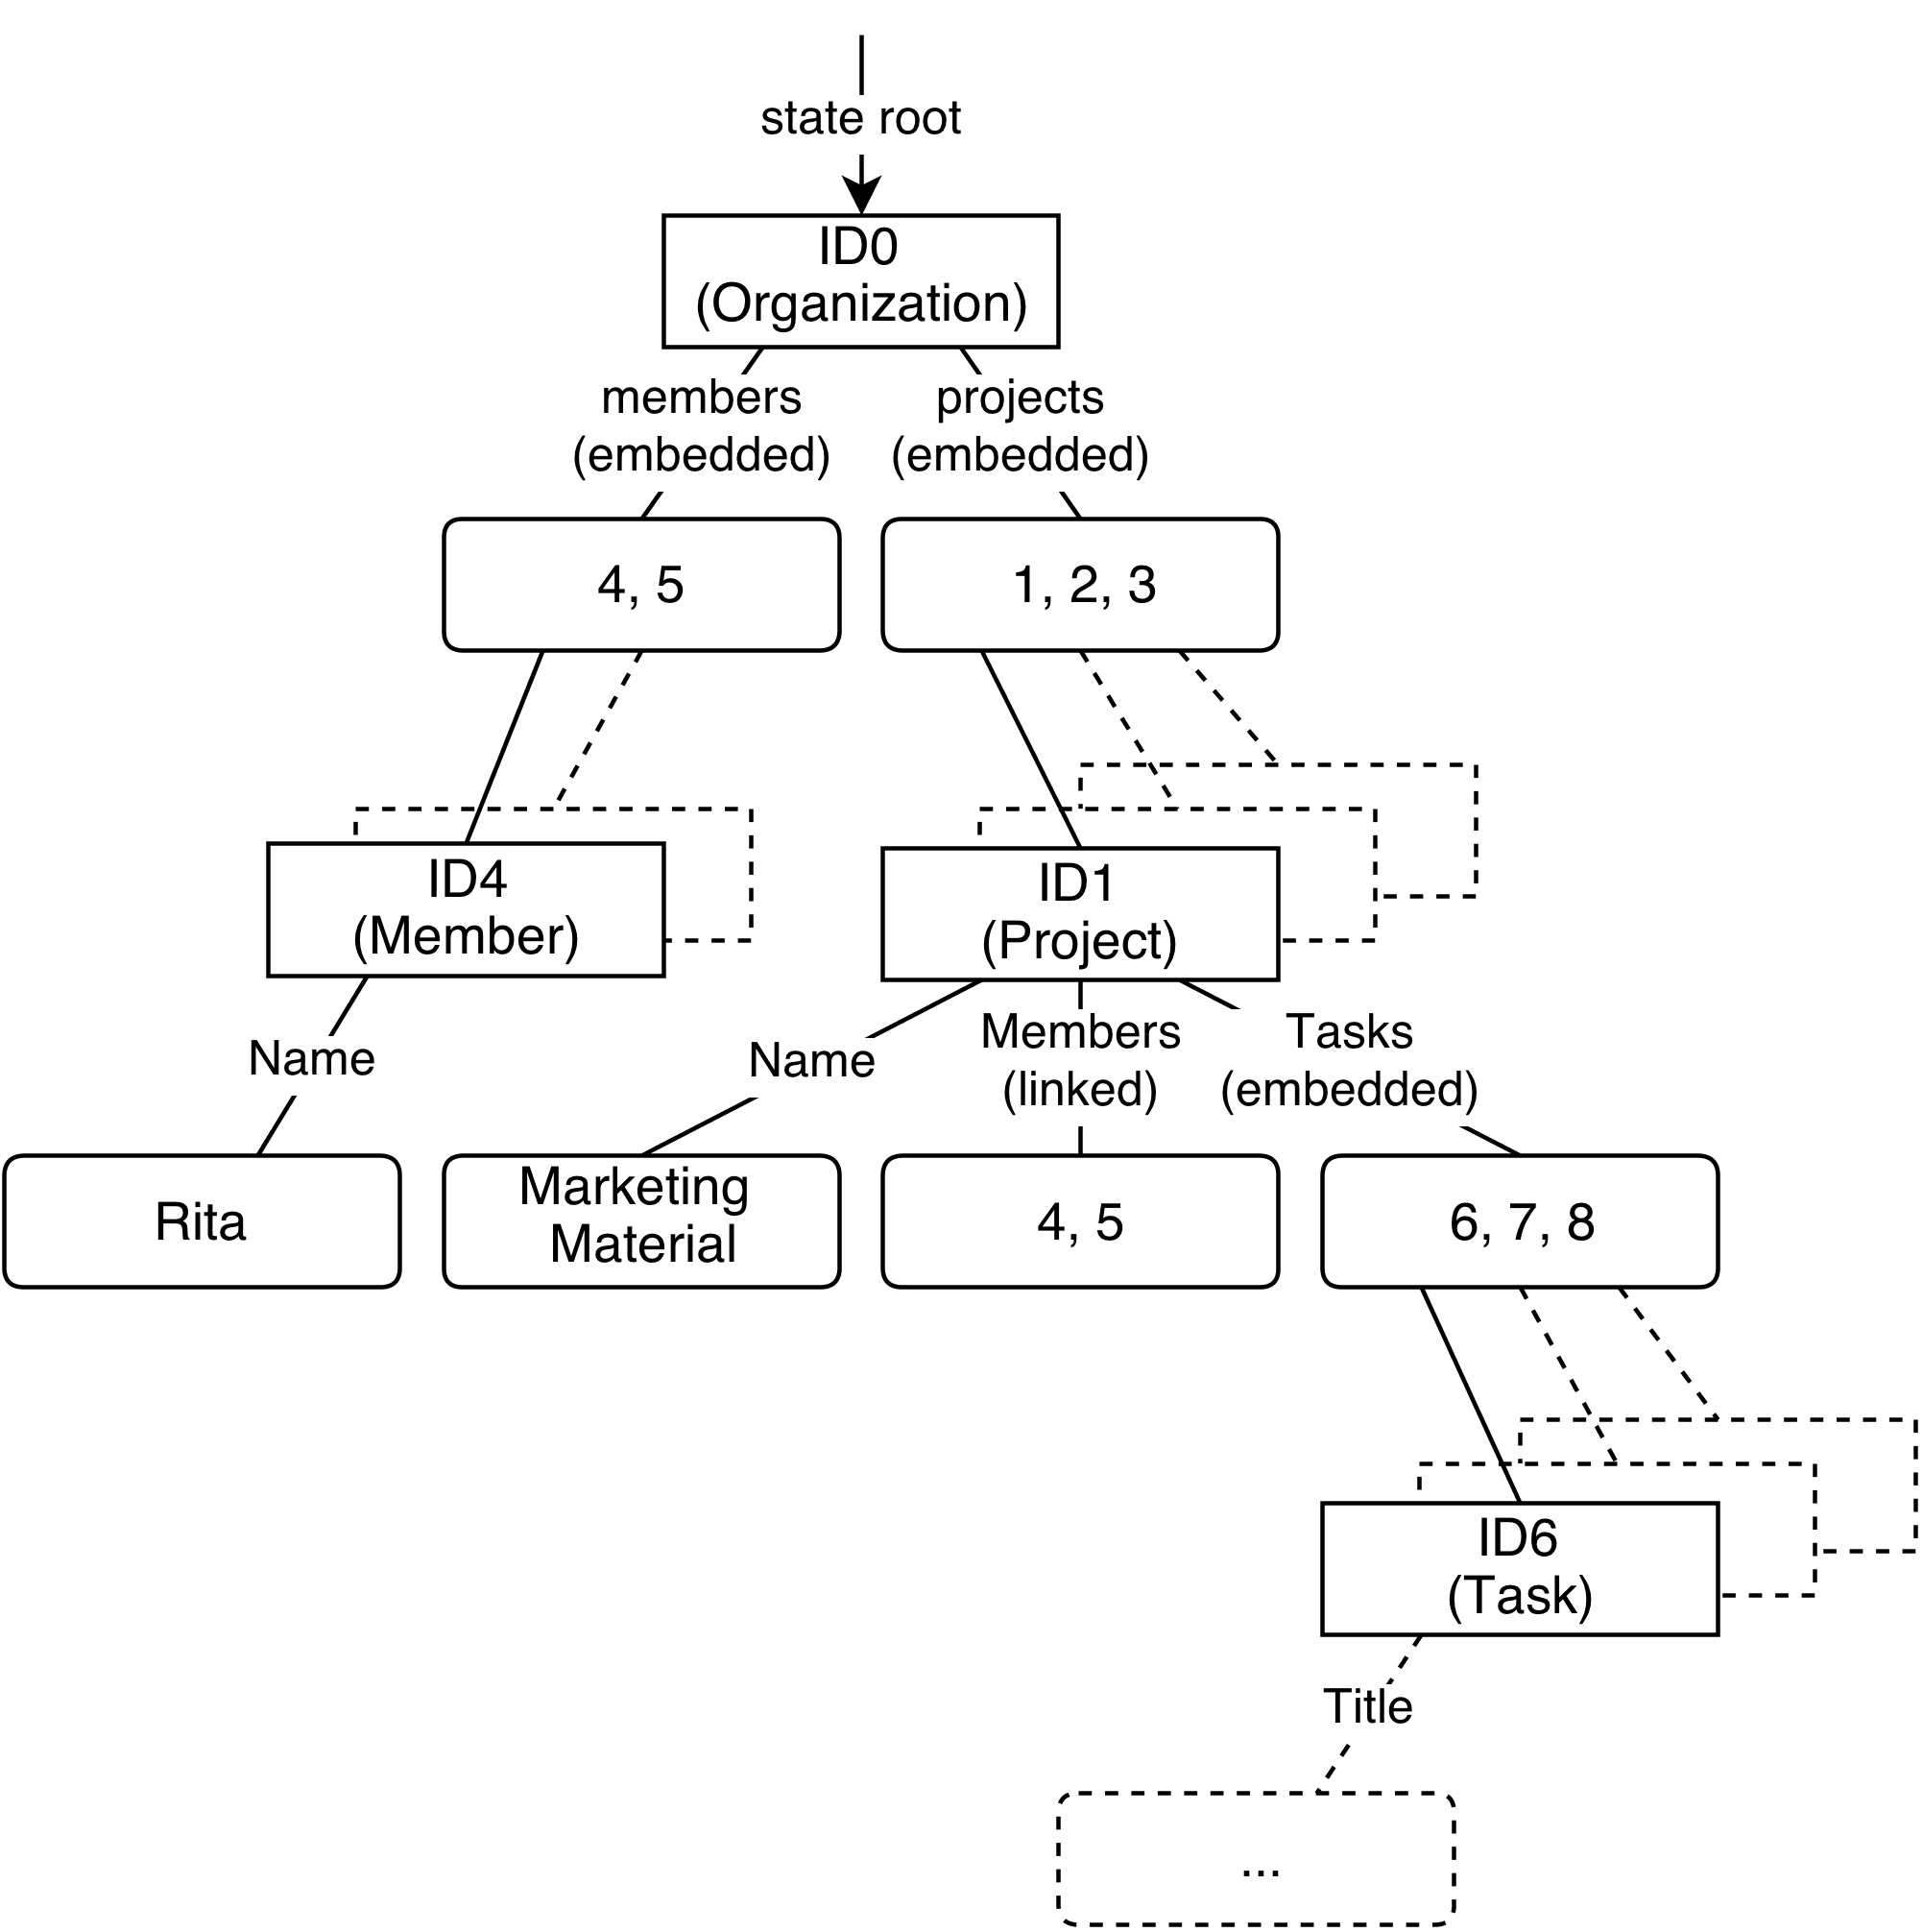
\includegraphics[width=0.8\textwidth]{img/hierarchy}
  \caption{The data model mapped to a hierarchy.}
  \label{fig:histo.hierarchy}
\end{figure}

Figure \ref{fig:histo.hierarchy} shows the actual hierarchy we derived from the data model in our scenario.

\section{Committing Objects}
We have seen how through the use of object embedding we can structure our data in a hierarchy.
When persisting our data we do not actually physically embed entire objects down the hierarchy.
If we did this we would end up with a single, big structure which would have to be re-written every time a small change was made.
We therefore store even embedded objects as separate structures.
At a logical level they are still embedded though - we achieve this through the use of cryptographic hashing.
All of our objects are stored in a content-addressable store which is described in section \ref{sec:background.cas}.
We can therefore retrieve each object based on a cryptographic hash of its content.
When logically embedding an object we actually save it in the store and only reference its hash.\\
Saving each object separately we can now re-use objects of previous states when new data is commited.
As shown in figure \ref{fig:histo.commits} each data update is represented through a new commit object.
Each commit object points to the root of the data hierarchy and therefore to a snapshot of the entire data.
Commit objects link to their parent commits and are therefore connected in a directed, acyclic graph.\\
Whenever an object in our graph changes, we only need to write the changed object and all its parents again.
All unchanged objects can be referenced again through their state hash.\\

Let us go through the steps of an exemplary update which could have lead to the scenario shown in figure \ref{fig:histo.commits}:

\begin{enumerate}
\item A new task with ID10 is added to project ID3 and committed.
\item Task ID10's state is written to the content-addressable store which returns its cryptographic hash.
\item Project ID3 which embeds Task ID10 references the new hash in its `tasks' attribute, Task ID9 is unchanged and can therefore be referenced without writing it again.\\
The new state of Project ID3 has to be written again returning its new hash.
\item Organization ID0 embeds Project ID3 and therefore has to update the hash in its `projects' attribute to the new version.\\
All other projects and entries of the `members' attribute can reference to the previous instance hashes without writing them again.
\item The new commit object links to the new hash of organization ID0 as the root object.
\item The new commit object links to the previous commit object.
\end{enumerate}

\begin{figure}[commits]
  \centering
  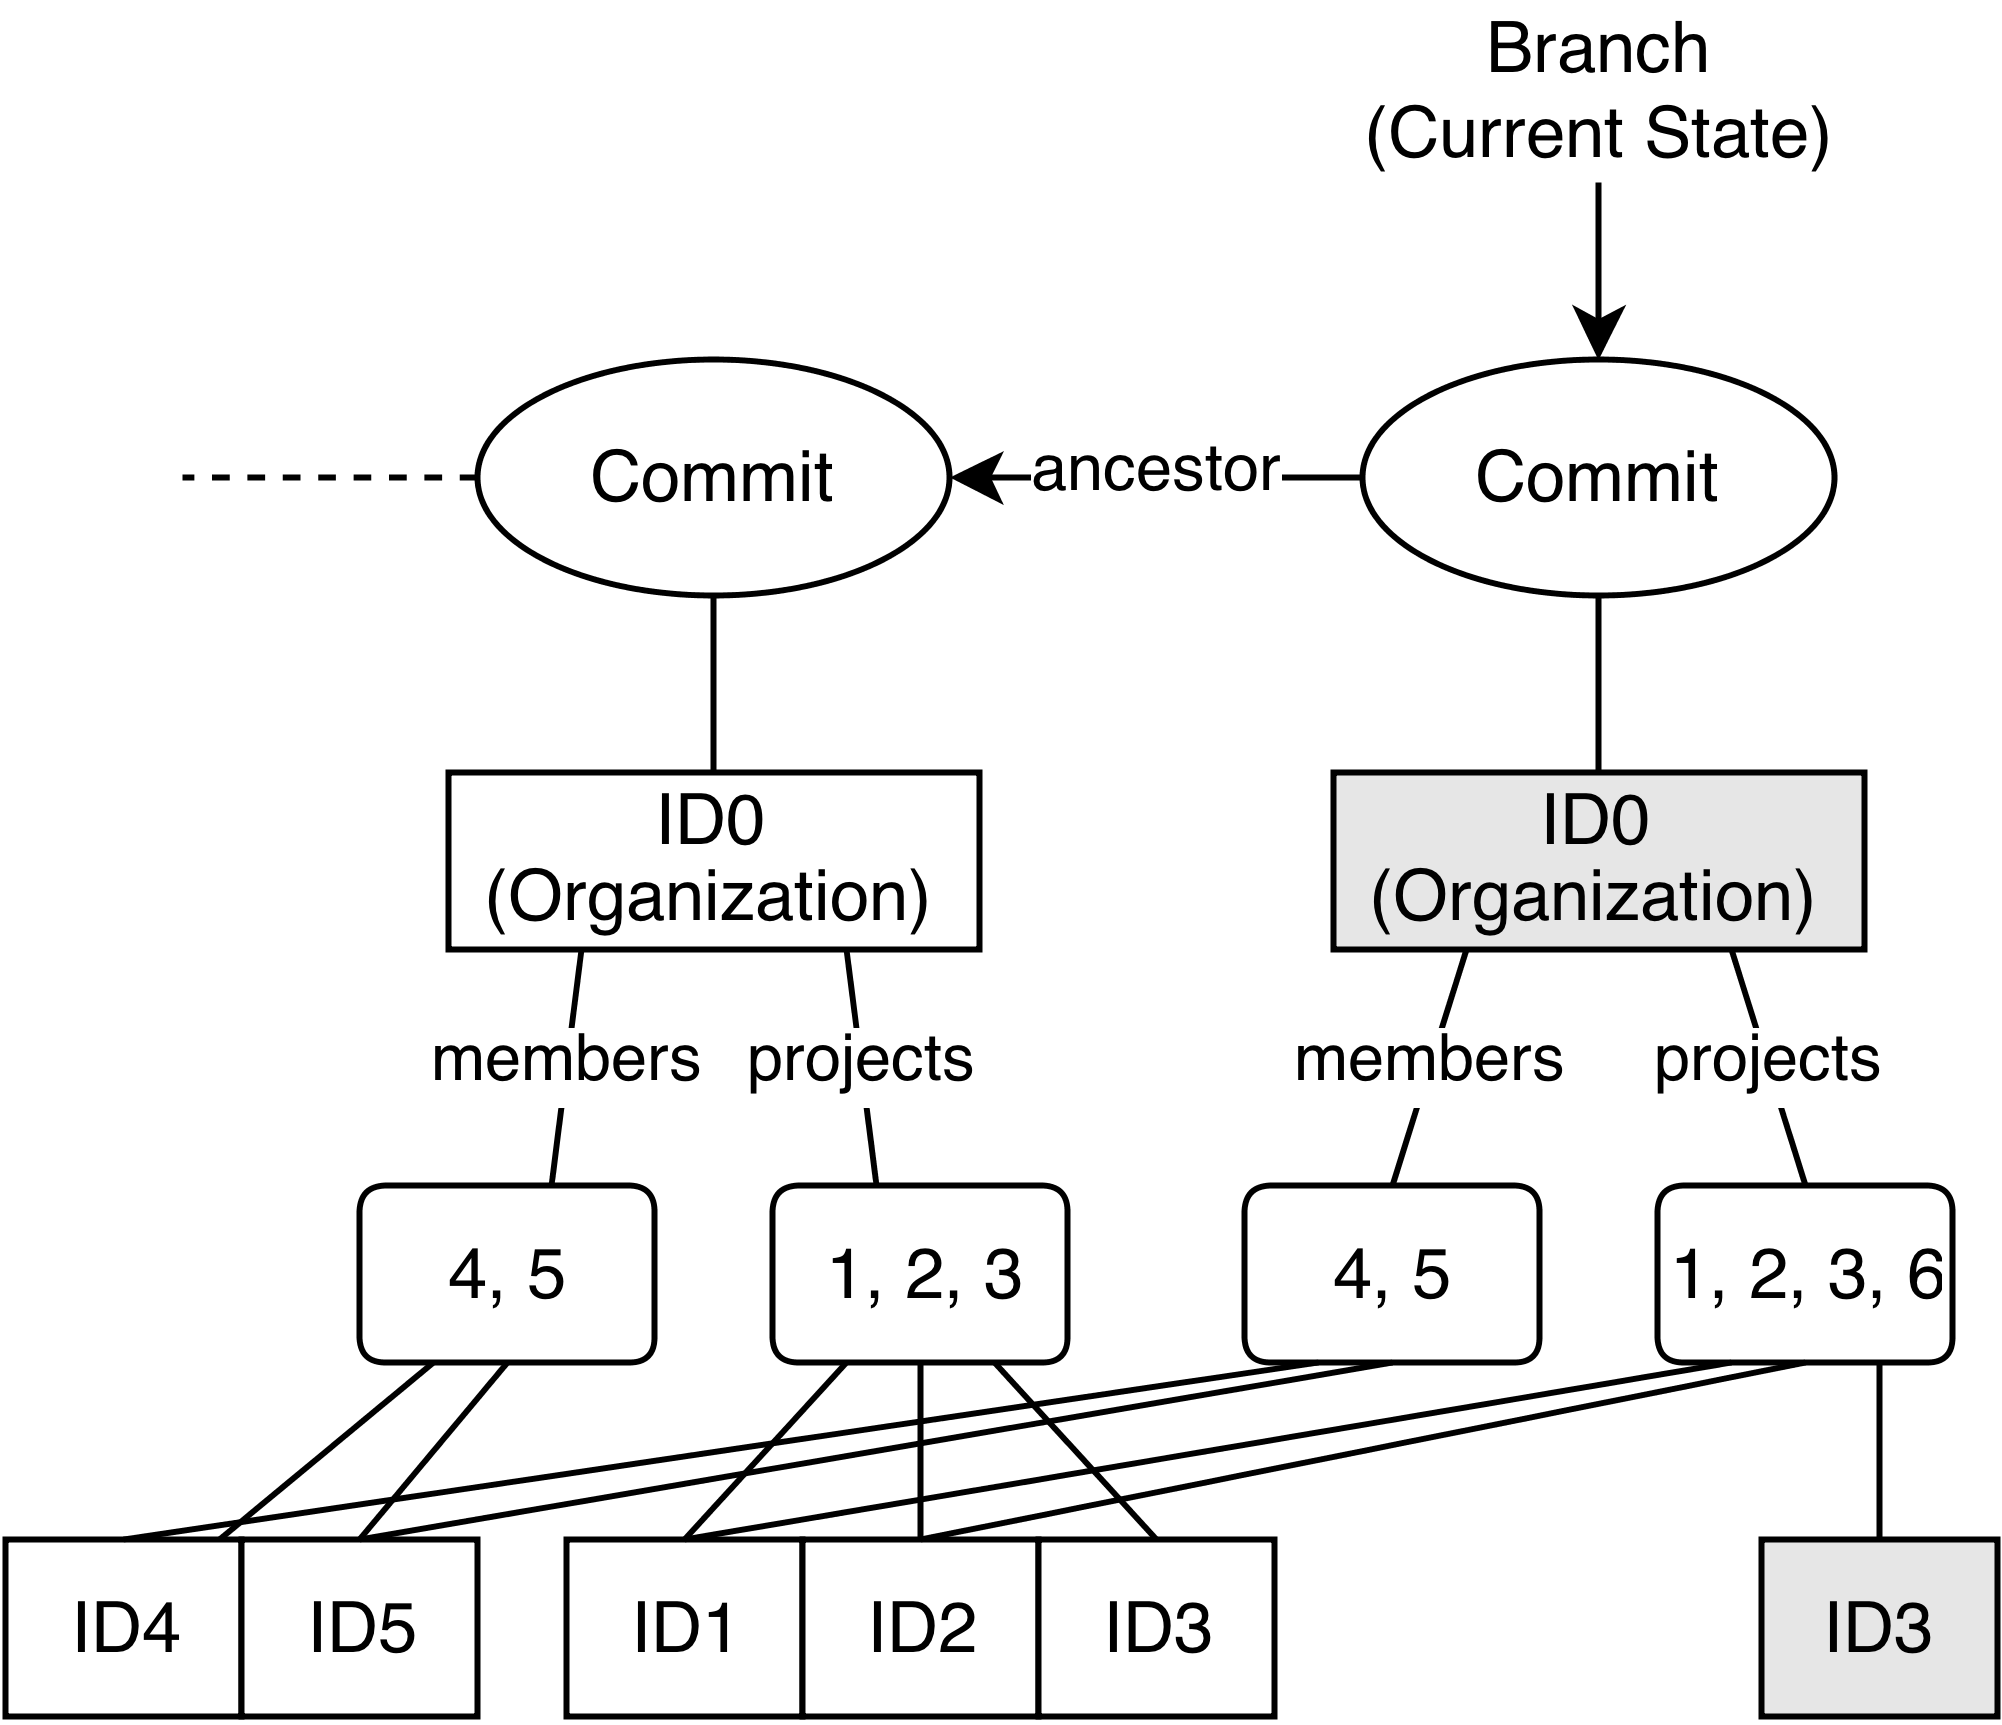
\includegraphics[width=0.6\textwidth]{img/commits}
  \caption{Re-using objects across commits.}
  \label{fig:histo.commits}
\end{figure}

With this model of hierarchical data at hand we can now go into the details of merging two branches of our state.

\section{Three-Way Merging of Objects}
\label{sec:main.histo.merging}
In this section we will focus on the core merging semantics which is part of the synchronization protocol developed in \ref{sec:main.protocol}.\\
As described in section \ref{sec:background.definition} synchronization always starts with an update detection phase.
Before we can start to merge branches we need to know about what has changed.
One our our design goals is to relieve the application developer from manual change tracing.
We therefore need to implement a differencing algorithm for the types of models described in section \ref{sec:main.requirements.data-models}.\\
We have described three-way merging as a general concept in section \ref{sec:background.merging}.
Our own algorithm will be structured into three types of algorithms.
Starting with a differencing phase we identify the changes made in two branches of our state B and C since our common ancestor state A.
Should an application decide to explicitly track changes it could actually leave this phase out and still benefit from the rest of our merging algorithm.\\
If follows a diff merging phase where the two diff results A-B and A-C are combined into one diff.
As its only input is the two diffs it does not require access to the actual states A, B or C.
In this phase we can have conflicts if the two branches contain updates to the same parts of the state.\\
The merged diff can then be applied to the origin state A in order to create the actual merged state.
For this step we require a patch algorithm.

Let us summarize the tree steps of the complete merge process of two branches:

\begin{itemize}
\item \textbf{Differencing}: we diff branch B and C with their common ancestor A.
\item \textbf{Merging}: we merge the two diffs A-B and A-C to a new diff result.
\item \textbf{Patching}: we apply the merged diffs as a patch to A which results in the merged state D.
\end{itemize}

\subsection{Diff and Merge Scenario}
\label{sec:main.histo.merging.scenario}
To show correctness of a merge algorithm we need to define sample model states with expected merge results.
This set of data can then be used as a test case for our implementation.
Based on an ancestor state all users start with, we define several possible branch states.\\
Merging of the branch states will happen on multiple levels of detail.
Each level will have its own difference and diff merge phase.
The result of the diff merge phases is then used to patch the common ancestor state.\\
Our common ancestor state A is described as the following:\\

\begin{tabular}{ l l l l }
\multicolumn{4}{ c }{\textbf{Ancestor state A of Projects}} \\
ID & Project Name & Members & Tasks \\
\hline
1 & Marketng Material & Rita, Tom, Allen & 1, 2, 3, 4 \\
2 & Product Roadmap & Rita, Allen & 5 \\
3 & Staffing & Rita & 9, 10\\
4 & Finances & Allen & 11
\end{tabular} \\

`Members' is an unordered collection of users - we define the user's IDs identical to their names.\\
`Tasks' is an ordered collection of tasks IDs.\\
We will leave out the details about other entities as the project instances already cover all required modeling aspects.\\

\begin{tabular}{ l l l l }
\multicolumn{4}{ c }{\textbf{State B of Projects}} \\
ID & Project Name & Members & Tasks \\
\hline
1 & Marketing Material & Rita, Tom & 1, 4, 2, 3, 6 \\
2 & Product Planning & Rita, Allen & 5 \\
3 & Staffing & Rita & 9, 10\\
4 & Finances & Allen & 11, 12\\
5 & Sales Planning & Rita, Tom & \\
\end{tabular} \\
\\

\begin{tabular}{ l l l l }
\multicolumn{4}{ c }{\textbf{State C of Projects}} \\
ID & Project Name & Members & Tasks \\
\hline
1 & Marketing Strategy & Rita, Tom, Allen & 4, 1, 2, 3 \\
2 & Product Strategy & Rita, Allen & 5, 7 \\
\end{tabular} \\
\\

We start the merging process at the highest level by computing the difference between the set of instances.
At this stage we are only interested in insert and remove operations of instances and in which instances have been updated.
We do not want to look at the differences between individual attribute values and therefore use the cryptographic hash of each instance.
Note that all hashes in this section are fictious to be easy to compare.\\

\begin{tabular}{ l l l l }
\multicolumn{4}{ c }{\textbf{Project Instance Set}} \\
ID & State A Hash & State B Hash & State C Hash \\
\hline
1 & 1A & 1AB & 1AC \\
2 & 2A & 2AB & 2AC \\
3 & 3A & 3A & - \\
4 & 4A & 4AB & - \\
5 & - & 5B & -
\end{tabular} \\
\\

\begin{tabular}{ l l l l }
\multicolumn{4}{ c }{\textbf{Project Instance Set Difference}} \\
ID & Diff A-B & Diff A-C & Diffs Merged \\
\hline
1 & update & update & conflict \\
2 & update & update & conflict \\
3 & - & remove & remove \\
4 & update & remove & conflict \\
5 & insert & - & insert
\end{tabular} \\
\\

Whenever the hash of an instance has only changed in one state, we carry the change over into the result.
If the hash has changed in both states, we have a conflict.
We will try to resolve conflicts by running a finer grained merge on the conflicting instance states.
ID 1 and 2 will therefore go into a lower level of merging while the changes in ID 3 and 5 are already accepted.
We cannot run the finer grained merge on ID 4 as it was removed in state C.
This conflict is therefore already carried over into the result.\\

Lets see if we can resolve conflicts 1 and 2 in the next merge.
At this level we will look at the actual instance data to find out which attributes are actually affected by the updates.
We will again use cryptographic hashes - this time to represent the attribute values:\\

\begin{tabular}{ l l l l }
\multicolumn{4}{ c }{\textbf{Attribute Value Hashs of ID 1}} \\
Attribute & State A Hash & State B Hash & State C Hash \\
\hline
Project Name & 1pA & 1pAB & 1pAC \\
Members & 1mA & 1mAB & 1mA \\
Tasks & 1tA & 1tAB & 1tAC
\end{tabular}\\
\\

\begin{tabular}{ l l l l }
\multicolumn{4}{ c }{\textbf{Attribute Value Difference of ID 1}} \\
Attribute & Diff A-B & Diff A-C & Diffs Merged \\
\hline
Project Name & update & update & conflict \\
Members & update & - & update \\
Tasks & update & update & conflict
\end{tabular}\\
\\

At this level we can already carry over the update of the `Members' attribute in B to the result.\\
The `Project Name' and `Tasks' attributes of B and C have still conflicting states.
If we define string values as atoms we have reached the most detailed level of merging - the conflict will therefore be carried over into the result.
If we instead see strings as another substructure we can attempt to resolve the conflict by using a string merging algorithm.\\
We have defined the `Tasks' attribute as an ordered set of instance IDs.
We can therefore try to resolve the conflict by applying a merge algorithm for ordered sets.\\

The result we expect from merging the `Project Name' strings:\\

\begin{tabular}{ l l l }
\multicolumn{3}{ c }{\textbf{`Project Name' of ID 1}} \\
State A & State B & State C\\
\hline
Marketng Material & Marketing Material & Marketing Strategy
\end{tabular}\\
\\

Note that all index positions in the following diffs are seen as relative to the ancestor state.
So even if one diff contains multiple insert or remove operations they are given as if they were all applied simultaneously to the ancestor state.\\

\begin{tabularx}{\textwidth}{ l X X }
\multicolumn{3}{ c }{\textbf{`Project Name' Difference for ID 1}} \\
Diff A-B & Diff A-C & Diffs Merged \\
\hline
insert `i' behind index 5 & insert `i' behind index 5 \newline remove from index 9 to 17 & insert `i' behind index 5 \newline remove from index 9 to 17
\end{tabularx}\\
\\

Applying this merge result to the ancestor state gives us an intuitive result: `Marketing Strategy'.\\

The expected output from merging the `Tasks' values looks similar:\\

\begin{tabular}{ l l l }
\multicolumn{3}{ c }{\textbf{`Tasks' of ID 1}} \\
State A & State B & State C \\
\hline
1, 2, 3, 4 & 1, 4, 2, 3, 6 & 4, 1, 2, 3
\end{tabular}\\
\\

\begin{tabularx}{\textwidth}{ X X X }
\multicolumn{3}{ c }{\textbf{`Tasks' Difference for ID 1}} \\
Diff A-B & Diff A-C & Diffs Merged \\
\hline
move index 3 behind index 0 \newline insert 6 behind index 3
& move index 3 behind index -1
& insert 6 behind index 3 \newline
conflict (`move index 3 behind index 0' and `move index 3 behind index -1')
\end{tabularx}\\
\\

We have been able to carry over one operation into the result while we still have an update conflict.
There is no way we can do an even finer grained merge to resolve this conflict.
The application developer will have to implement a custom merge solution - possibly even asking the user which operation to choose.\\
Depending on how the conflict is resolved, possible results are:

\begin{itemize}
\item 1, 4, 2, 3, 6
\item 4, 1, 2, 3, 6
\end{itemize}

The merge of ID 2 works analogous - we will therefore skip the attribute merging step and jump right into the string merge:\\

\begin{tabular}{ l l l }
\multicolumn{3}{ c }{\textbf{`Project Name' of ID 2}} \\
State A & State B & State C \\
\hline
Product Roadmap & Product Planning & Product Strategy
\end{tabular}\\
\\

\begin{tabularx}{\textwidth}{ X X X }
\multicolumn{3}{ c }{\textbf{`Project Name' Difference for ID 2}} \\
Diff A-B & Diff A-C & Diffs Merged \\
\hline
remove from index 8 to 15 \newline insert `Planning' behind index 7
& remove from index 8 to 15 \newline insert `Strategy' behind index 7
& remove from index 8 to 15 \newline insert `Planning' behind index 7
\newline insert `Strategy' behind index 7
\end{tabularx}\\
\\

We have applied the same merge logic that helped us resolve the conflict in ID 1.
But the result we get here is not what a user would expect.
Applying the merged operations to the ancestor state results in: `Product StrategyPlanning'.\\
This is a good example for the violation of intention preservation.
Both in state B and C the user actually intended to \emph{replace} the word `Roadmap'.
Concurrently replacing the same word should clearly cause a conflict.
Our differencing algorithm has no notion of a `replace' operation.
All it sees is a remove of `Roadmap' and an insert of some other word.\\
This example shoes the limits of generic merging algorithms that preserve user intention.\\
In practice it would propably be more suitable to define the `Project Name' as an atom.
As names are short it is more likely that an update is actually intended as a replace operation of the entire string.

\subsection{Differencing}
\label{sec:main.histo.merging.diff}
Differencing algorithms have been studied extensively.
There exist efficient solutions for a range of data structures.
It is not a focus of our thesis to develop the most efficient differencing algorithm matching our scenario.
Our goal in this section is to show the practical feasibility of the three-way merging component in our architecture.
We favor a simple solution, re-using existing concepts so that we can broaden our focus on an other areas of our synchronization solution.\\
The test case defined in the previous section can be decomposed and mapped to common data structures.\\
The first merging level of instances represented as cryptographic hash can be mapped to a \emph{dictionary} with key-value entries.\\
Same is true for instance-level merging: the dictionary keys are mapped to the attribute names and the dictionary values to the respective value hashs.\\
Attribute values that represent collections of instance IDs can be mapped to \emph{sets}.
Our `Members' attribute does not have a relevant order, it can be mapped to an ordinary set.
The `Tasks' attribute has a significant order and therefore has to be mapped to an \emph{ordered set}.\\
If we do not treat string values as atoms we have to represent them as an \emph{ordered list}.\\

To summarize - for the following data structures we need an algorithm that finds the difference from an origin state A to a changed state B:

\begin{itemize}
\item \textbf{Dictionaries}: to model entity instances and instance attributes.
\item \textbf{Sets and Ordered Sets}: to model instance relationships.
\item \textbf{Ordered Lists / Strings}: to model string values of instance attributes.
\end{itemize}

Ordered list or string data structures have been the main focus in previous research on difference algorithms.
Myers presented an efficient algorithm with $\mathcal O(n*d) $ time and space complexity to difference two strings A and B with
$ n $ representing the sum of the lengths of two strings and $ d $ the size of the shortest edit script transforming A to B \cite{Myers:1986wi}.
The shortest edit script is equivalent to the result of a differencing algorithm.
As in practical applications differences are usually small the algorithm performs well.\\

Given the ordered list difference algorithm we can re-use it to build an algorithm for ordered sets.
Ordered lists can only have differences in the form of \emph{insert} or \emph{remove} operations.
Ordered sets extend this - the simultaneous remove and insert of a globally unique element is now considered as a move operation.\\
To implement an ordered set algorithm we can therefore take the output of the ordered list algorithm and scan the result for the remove and insert of the same element.
This can be efficiently implemented through a hash:

\begin{enumerate}
\item Scan the diff result and build a hash for all removed elements.
\item Scan the result again and test for all inserted elements whether they are included in the hash.
\item If a match is found replace the remove and insert operations through a single move operation in the result.
\end{enumerate}

The time complexity of building a hash can be estimated with $ \mathcal O(n * log(n)) $ with $ n $ representing set size.
The match searching has linear time complexity.
We therefore only add $ \mathcal O(n * log(n)) $ complexity to Myers difference algorithm for a naive solution for ordered sets.\\

For ordinary sets we can implement a simple solution through two hashs of the respective set entries combined with a scan through each set:

\begin{enumerate}
\item Add all entries of set A to a hash $ H_A $ and those of set B to a different hash $ H_B $.
\item Scan set A and test for matches in hash $ H_B $.
\item If no match is found add a remove operation to the result.
\item Scan set B and test for matches in hash $ H_A $.
\item If no match is found add an insert operation to the result.
\end{enumerate}

\emph{Insert} and \emph{remove} are the only operations in a set.\\
The time complexity for building each hash is again $ \mathcal O(n * log(n)) $.
Searching for matches has linear complexity which results in a time complexity $ \mathcal O(n * log(n)) $ for the entire algorithm.\\

A dictionary data structure has \emph{insert}, \emph{remove} and \emph{update} operations.
If the instance described through the dictionary has a fixed set of attributes it would actually only need to support an update operation.
In modern web applications it is not uncommon that there is no fixed data schema.
It is often the case that new attributes are added to instances at runtime.
Even if there is a fixed schema it might be changed through a software update with old instances not being migrated to the new schema.
We should therefore support the full set of dictionary operations in our difference algorithm.

A simple and efficient solution is to again use two hashes for fast lookup combined with a scan through both dictionaries:

\begin{enumerate}
\item All all keys and values of dictionary A to hash $ H_A $ and those of dictionary B to hash $ H_B $.
\item Scan through all key-value entries of A.
\item If the key is not included in hash $ H_B $, add a remove operation to the result.
\item If the key is included and the value in $ H_B $ is different, add an update operation.
\item Scan through all key-value entries of B.
\item If the key is not included in hash $ H_A $, add an insert operation to the result.
\end{enumerate}

Building the hash is again estimated with time complexity $ \mathcal O(n * log(n)) $, scanning both dictionaries has linear time complexity. The combined time complexity is therefore again $ \mathcal O(n * log(n)) $.\\
Depending on the application, its instances are often already implemented with hash-like lookup performance - in this case we could skip step 1.
The time complexity is in this case only linear.\\

\subsection{Diff Merging}
\label{sec:main.histo.merging.merge}

We will now look into strategies for merging the diff results of the algorithms described in the previous section.
Our focus lies on the identification of potential conflicts based on three-way merging semantics.\\

Ordered lists only support insert and remove operations.
Concurrent insert or remove operations are never conflicting as they do not update existing structures.
As we have seen in the example at the end of section \ref{sec:main.histo.merging.scenario} this is not necessarily in line with a user's intentions.
When editing text users often intend to \emph{replace} content although their actions are represented through a remove and insert operation.
This is why most concurrent version control systems have the notion of \emph{areas} in text.
Concurrent insert or remove operations in overlapping areas are considered as update operations to the same content and therefore result in conflicts.\\
The optimal definition of an area can vary depending on the application.
It may be the entire edited paragraph, a number of lines, sentences, words or even characters.\\
When modeled as an ordered list we can only vary the number of list elements defining the size of an area.\\
Concurrent insert or remove operations which are not in overlapping areas are simply both carried over to the merge result.\\

Ordinary sets have the same operations as ordered lists except that each element is unique and we now have no element order.
Without a specified order we can not define \emph{areas}.
Merging two diffs is therefore trivial as no conflicts can occur.
We simply combine the set of operations of both diffs into one large diff.\\

Ordered sets add move operations as we can uniquely identify each element.
Move operations can lead to conflicts if the same element is concurrently moved to different locations.
If move operations are not conflicting they are carried over into the merge result.
Insert and remove operations are merged the same way as defined for ordered lists.\\

Dictionaries have insert, remove and update operations.
Concurrent insert and remove operations never lead to conflicts - they are carried over into the merge result.
Update operations can lead to conflicts if the value of the same key is concurrently modified.

\subsection{Patching}
\label{sec:main.histo.patching}

Patching is defined as an algorithm applying the identified differences between state A and B as operations to state A.
A computed diff A-B patched to A will result in B.
For our three-way merging algorithm, patching constitutes the last phase. 
Two merged diffs are applied as a patch to the common ancestor state resulting in the actual merged state.\\
We again need patching algorithms for each data structure we intend to support.
The implementation needs to consider that simply executing the operations defined in the diff can lead to a wrong result.
This is true if a change operation has side effects on other parts of the state.\\
In our set of data structures this is only the case for ordered lists and ordered sets.
Applying an insert operation at the specified index, renders the indexes of following operations wrong.
A simple example:

\begin{itemize}
\item State A: `Marketng Matrial'
\item Diff:\\
insert `i' behind index 5\\
insert `e' behind index 11
\end{itemize}

Applying the first diff operation to A results in: `Marketing Matrial'.\\
If we now execute the second operation at the specified index 11 we get: `Marketing Maetrial'.\\
The implementation therefore needs to treat the given indexes as relative positions in the ancestor state.\\
The diff operations of sets and dictionaries can be executed as they are without taking side-effects into consideration.

\subsection{Hierarchical Merging}
As we have seen in our scenario, merging of our structured data is actually a hierachical process combining all of the described algorithms.
Our strategy is to start at the highest-level representing sub-structures using their cryptographic hash.
Whenever we identify an update on the hash of a sub-structure we do a finer grained diff and merge on the structure itself:

\begin{enumerate}
\item Represent all instances of an entity as a dictionary with instance IDs as keys and a cryptographic hash of their attribute values as dictionary values.
\item Use the dictionary diff algorithm to identify inserted, removed and updated instances on A-B and A-C.
\item Merge the dictionary diffs to result \emph{M1}.
\item Remove each instance with an update conflict from \emph{M1}.\\
Represent it as a dictionary with keys being attribute names and values being a cryptographic hash of attribute values.
\item Use the dictionary diff algorithm to identify inserted, removed and updated attributes.
\item Merge the per-instance diffs to result \emph{M2}.
\item Remove each non-atomic attribute with an update conflict from \emph{M3}.\\
Run the respective algorithm:\\
Attributes with (ordered) sets of instance IDs: (ordered) set diff algorithm.\\
Attributes with string values: ordered list diff algorithm.
\item Merge the attribute diffs to result \emph{M3}.
\item Resolve all remaining conflicts in \emph{M1}, \emph{M2} and \emph{M3} manually.
\item Patch the respective substructures of state A using \emph{M1}, \emph{M2} and \emph{M3}.
\end{enumerate}

This approach can not only be applied to difference entity-relationship models, it can actually be adapted for any type of data with a hierarchical structure.

\section{Commit Changes Stream}
\label{main.diff-across-commits}

TODO:

- write each commit to a changes stream similar to couchdb

- peer nodes can listen in real-time

\section{Synchronization Protocol}
\label{sec:main.protocol}
Synchronization always happens from a \emph{Source} node to a \emph{Target} node.
If it is run simultaneously with Source and Target exchanged, it keeps both nodes in sync with each other.\\
The algorithm is designed to be able to run independently of the Source or Target.
It could be implemented as a separate application possibly even running on a different device - as long as it has access to both the Source and Target node.\\
The Synchronizer could be run in regular intervals or explicitly triggered by changes in the Source node.\\

The latest commit on a node we refer to as the \emph{head}.
A node has a \emph{master head} which refers to the version of the data considered to be `true' by the node.\\
For each remote node it synchronizes with, the node keeps a \emph{remote tracking head}.\\
A remote tracking head represents what the local node considers to be the current state of a remote node.

Synchronization follows a two-step protocol, step one propagates all changed data from Source to Target, step two executes a local merge operation.

\subsubsection{Propagation}
Propagation follows the following protocol:

\begin{enumerate}
\item Read all commit IDs since the last synced commit from Source and write them to Target.
\item Let the Target compute the common ancestor commit ID of Target's and Source's master heads.
\item Read all changed data since the common ancestor commit from Source and write to Target.
\item Set the Target's remote tracking head of Source to Source's master head.
\end{enumerate}

Once these steps are executed, the Target node has the current state of Source available locally.\\
The Target's head still refers to the same state as the Source data has not been merged.\\

Listing \ref{propagation-protocol} summarizes the protocol as pseudo-code.

\begin{lstlisting}[caption=Propagation Protocol, label=propagation-protocol]

commitIDsSource = source.getCommitIDsSince(lastSyncedCommit)

target.writeCommitIDs(commitIDsSource)

commonAncestor = target.getCommonAncestor(target.head.master, source.head.master)

changedData = source.getChangedDataSince(commonAncestor)

target.writeData(changedData)

\end{lstlisting}

The functions `getCommitIDsSince()' and `getChangedDataSince()' are implemented as described in section \ref{main.diff-across-commits}.\\
The most recent common ancestor algorithm used in `getCommonAncestor()' is described in section \ref{background.mrca}.\\
The internals used by `writeData()' and the underlying commit data model are explained in section \ref{main.committing}.

\subsubsection{Merging}
Even if the Source is disconnected at this stage, the Target has all the necessary information to process the merge offline:\\

\begin{itemize}
\item The Target's master head we refer to as the \emph{master head}.\\
\item The Target's remote tracking branch for the Source we refer to as the \emph{Source tracking head}.
\end{itemize}

\begin{enumerate}
\item Compute the common ancestor of the master head and the Source tracking head. (The common ancestor could also be re-used from the propagation step.)
\item If the common ancestor equals the Source tracking head:\\
  The Source has not changed since the last synchronization. The master head is ahead of the Source tracking head.\\
  The algorithm can stop here.
\item If the common ancestor equals the master head:\\
  The Target has not changed since the last synchronization.\\
  The Source's head is ahead of Target.\\
  We can fast-forward the master head to the Source tracking head.
\item If the common ancestor is neither the Source tracking head nor the master head:\\
  Both Source and Target must have changed data since the last synchronization.\\
  We run a three-way merge of the common ancestor, Source tracking head and master head.\\
  We commit the result as the new master head.
\end{enumerate}

This protocol is able to minimize the amount of data sent between synced
stores even in a distributed, peer-to-peer setting.\\

Updating the Target's head uses optimistic locking.
To update the head you need to include the last read head in your request.
So both the fast-forward operation or the commit of a merge result can be rejected if the Target has been updated in the meantime.
If this happens the Synchronizer simply has to re-run the merge algorithm.\\

The merging process can be described in pseudo-code as shown in figure \ref{merging-protocol}.

\begin{lstlisting}[caption=Merging Protocol, label=merging-protocol]

masterHead = target.head.master
sourceTrackingHead = target.head.sourceID

commonAncestor = target.getCommonAncestor(masterHead, sourceTrackingHead)

if (commonAncestor == sourceTrackingHead) {
  // do nothing

} else if (commonAncestor == masterHead) {
  // fast-forward master head
  try {
    // when updating the head we have to pass in the previous head:
    target.setHead(sourceTrackingHead, masterHead)
  } catch {
    // the master head has been updated in the meantime
    // start over
  }

} else {
  commonAncestorData = target.getData(commonAncestor)
  sourceHeadData = target.getData(sourceTrackingHead)
  targetHeadData = target.getData(masterHead)

  mergedData = three-way-merge(commonAncestorData, sourceHeadData, targetHeadData)

  // commit object linking commit data with its ancestors:
  commitObject = createCommit(mergedData, [masterHead, sourceTrackingHead])

  try {
    // when updating the head we have to pass in the previous head:
    target.commit(commitObject, masterHead)    
  } catch {
    // the master head has been updated in the meantime
    // start over
  }
}

\end{lstlisting}

\section{Handling Conflicts}

TODO:

- application specific, no general solution

- automatic resolution strategies

- manual resolution through user

\section{Synchronization Topologies}

TODO:

- document different supported topologies

- client-server

- client-client

- client-server + server-server

- hierarchical (office server + cloud server)

\section{Optimizations}

TODO:

- Only keep limited history.

- Clients who are disconnected for too long have to fetch redundant data.

- Ideal case: remember until oldest head of nodes.

\section{Integration with Application Logic}

TODO:

- demonstrate how to interface with standard MVC frameworks like Backbone, Ember.js, Angular
